\documentclass[11pt]{enpc-article}

\usepackage{mathrsfs}
\usepackage{siunitx}
\usepackage{enumitem}

\title{\vspace{-2em}Deep Learning for Natural Language Processing}
\author{Louis \textsc{Trezzini}}
\date{\today}

\def\lb{\left[}
\def\rb{\right]}
\def\lp{\left(}
\def\rp{\right)}

\usepackage[title]{appendix}
\usepackage{array}

\begin{document}
\maketitle

\setcounter{section}{1}

\section{Multilingual word embeddings}

\subsection*{Question}

We want to minimize $\norm{W X - Y}$ under the constraint that $W \in O_d(\mathbb{R})$.

We notice :
\begin{align*}
  \norm{W X - Y}_F^2
  &= \langle W X - Y, W X - Y \rangle \\
  &= \norm{W X}_F^2 + \norm{Y}_F^2 - 2 \langle W X, Y \rangle \\
  &= \norm{X}_F^2 + \norm{Y}_F^2 - 2 \langle W X, Y \rangle
\end{align*}

So minimizing $\norm{W X - Y}$ is equivalent to maximizing $\langle W X, Y \rangle$.

Let's write $U \Sigma V^T = SVD(Y X^T)$. We have :
\begin{align*}
  \langle W X, Y \rangle
  &= \langle W, Y X^T \rangle \\
  &= \langle W, U \Sigma V^T \rangle \\
  &= \langle U^T W V, \Sigma \rangle
\end{align*}

Let's denote $Q = U^T W V$. We have :
\begin{align*}
  \langle Q, \Sigma \rangle
  &= \text{Trace}(Q^T \Sigma) \\
  &= \sum_{k = 1}^{d} Q_{kk} \Sigma_{kk}
\end{align*}

Because $\Sigma$ is diagonal.

Notice that $Q = U^T W V \in O_d(\mathbb{R})$ because $O_d(\mathbb{R})$ is a group and $U, V, W$ belong to it. It implies that $Q_{kk} \in [-1,1]$.

Thus, this expression is maximized when $Q = I$, since we need to choose $Q_{kk}=1$ for all $k$ because the entries of $\Sigma$ are non-negative.

So :
$$
  Q = I \Leftrightarrow U^T W V = I \Leftrightarrow W = U V^T
$$

\section{Sentence classification with BoV}

\subsection*{Question}

\section{Deep Learning models for classification}

\subsection*{Question 1}

I used the categorical cross-entropy loss.

Its formula is

$$
  - \frac{1}{N} \sum_{i = 1}^N \sum_{c = 1}^C \mathbf{1}_{\{y_i = c \}} \log(p(\hat{y_i} = c))
$$

where $N$ is the number of examples, $C$ is the number of classes, $y_i$ is the true label of example $i$, and $\hat{y_i}$ is the predicted label of example $i$.

\subsection*{Question 2}

\begin{figure}[H]
  \centering
  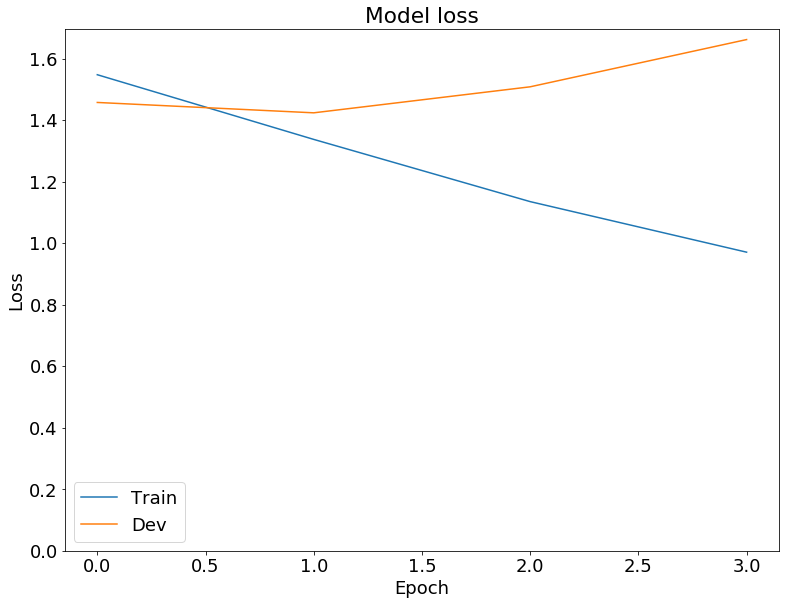
\includegraphics[width=\textwidth]{learning_curve.png}
  \caption{Evolution of train/dev results w.r.t the number of epochs.}
\end{figure}

\subsection*{Question 3}


\end{document}
